\documentclass[conference]{IEEEtran}
\IEEEoverridecommandlockouts
\usepackage{cite}
\usepackage{amsmath,amssymb,amsfonts}
\usepackage{algorithmic}
\usepackage{graphicx}
\usepackage{textcomp}
\usepackage{xcolor}
\usepackage{float}
\usepackage{subcaption}
\usepackage{multirow}
\usepackage{tabularx}
\def\BibTeX{{\rm B\kern-.05em{\sc i\kern-.025em b}\kern-.08em
    T\kern-.1667em\lower.7ex\hbox{E}\kern-.125emX}}
\begin{document}

\title{Enhancing Cardiovascular Risk Prediction Using Support Vector Machines and Advanced Machine Learning Algorithms}

\author{\IEEEauthorblockN{1\textsuperscript{st} Abhijit Pathak}
\IEEEauthorblockA{\textit{Assistant Professor} \\
\textit{BGC Trust University Bangladesh}\\
Chattogram, Bangladesh \\
abhijitpathak@bgctub.ac.bd \\
0000-0001-7734-0271}
\and
\IEEEauthorblockN{2\textsuperscript{nd} Touhidul Alam Seyam}
\IEEEauthorblockA{\textit{Research Assistant} \\
\textit{BGC Trust University Bangladesh}\\
Chattogram, Bangladesh \\
touhidulalam@bgctub.ac.bd \\
0009-0007-7512-1893}
\and
\IEEEauthorblockN{3\textsuperscript{rd} Arnab Chakraborty}
\IEEEauthorblockA{\textit{Research Assistant}\\
\textit{BGC Trust University Bangladesh}\\
Chattogram, Bangladesh \\
arnabchakrabortybd@gmail.com\\
0009-0008-0279-7187}
\and
\IEEEauthorblockN{4\textsuperscript{th} Nurjahan kamal Santa}
\IEEEauthorblockA{\textit{Research Assistant} \\
\textit{BGC Trust University Bangladesh}\\
Chattogram, Bangladesh \\
nurjahankamalsanta@gmail.com \\
0009-0009-7420-1255}
\and
\IEEEauthorblockN{5\textsuperscript{th} Eftakar Uddin}
\IEEEauthorblockA{\textit{Research Assistant} \\
\textit{BGC Trust University Bangladesh}\\
Chattogram, Bangladesh \\
eftakarjm03@gmail.com \\
0009-0001-3482-592X}
\and
\IEEEauthorblockN{6\textsuperscript{th} Tasmim Akther Mim}
\IEEEauthorblockA{\textit{Research Assistant}\\
\textit{BGC Trust University Bangladesh }\\
Chattogram, Bangladesh\\
tasmoomim@gmail.com\\
0009-0008-2787-0045}
}

\maketitle

\begin{abstract}
    A major cause of illness and mortality on a global scale is Cardiovascular Disease (CVD). Ensuring timely response and efficient management requires precise risk prediction. This study rigorously examines the use of support vector machines (SVM) and other advanced machine learning algorithms to optimize cardiovascular risk prediction. The authors have obtained a comprehensive dataset comprising patient gender analysis, patient behavior, and medical history parameters from a diverse patient cohort. The dataset has been meticulously preprocessed to impute missing values and accurately welcome and encode attributes. The authors utilized multiple machine learning models, including SVM, random forest, and XG boosting, to forecast the likelihood of future cardiovascular events. The authors' results unequivocally demonstrate that SVM, with its kernel technique and margin optimization, delivers superior performance in accuracy, precision, and recall compared to traditional logistic regression models. Ensemble methods such as Random Forest and XG Boosting are essential for managing imbalanced data and performing thorough feature importance analysis in data science and machine learning. This will enable doctors to easily understand each feature in predicting risk. In conclusion, the integration of machine learning algorithms, especially SVMs, into cardiovascular risk prediction frameworks can significantly enhance their predictive power. These advances have the potential to revolutionize CVD risk stratification and pave the way for personalized medicine, ultimately improving patient outcomes.
\end{abstract}

\begin{IEEEkeywords}
    Cardiovascular Risk Prediction, Support Vector Machines, Machine Learning, Clinical Data Analysis, Model Interpretability, Personalized Medicine.
\end{IEEEkeywords}

\section{Introduction}
Cardiovascular diseases (CVDs) are a considerable public health challenge globally and contribute significantly to the prevalence of mortality and morbidity in the world. Prevention of CVD and successfully managing a person's risk of CVD require knowing and predicting one's risk of CVD. Risk factors have been defined as modifiable (such as diet, physical activity, smoking) or non-modifiable (such as age, sex, and family history). Most of the current risk assessment models like the Framingham Risk Score, offer valuable insights but do not capture the intricate interplay between the range of factors that impact cardiovascular health. With the advancements in machine learning, the prediction of CVD risk has shown promise in providing increased satisfactory prediction and reliability and enhancing the accuracy and reliability of cardiovascular disease risk prediction, to promote better outcomes and apply targeted preventive strategies. Particularly, Support Vector Machines (SVMs) have shown promise in managing high-level data and identifying complex non-linear correlations. Also, an array of machine learning tools consisting of Random Forest, Gradient Boosting, Neural Networks, and others showed promise in various prediction tasks. In the prediction of cardiovascular disease risks, traditional models are widely employed. Traditional models, however, have limitations in modeling interactions and can only handle simple linear relationships thus proving difficult in predicting the cardiovascular risk. We need to develop cardiovascular risk prediction algorithms that have higher accuracy and reliability to allow for the early identification and treatment of an individual’s cardiovascular health risk. The potential for machine learning algorithms like Support Vector Machines in predicting cardiovascular risk offers a potential advance over traditional techniques. This research will evaluate several objectives:
\begin{enumerate}
    \item Evaluation of the predictive accuracy of SVM in comparison with traditional techniques for predicting cardiovascular risk.
    \item Compare the performance of support vector machines (SVMs) with other state-of-the-art machine learning algorithms, such as gradient boosting, random forest, and artificial neural networks.
    \item Evaluate the overall predictive performance of the machine learning models against classical models.
    \item Ensure that we deploy large and diverse datasets to ensure robust, generalizable results.
    \item The authors aim to contribute to the development of more precise and personalized tools for cardiovascular risk prediction, to provide an early risk signal, and to optimize resource allocation.
\end{enumerate}
Overall, our research aims to improve patient outcomes, optimize healthcare costs, and significantly increase the worldwide applicability of cardiovascular risk prediction models, which will contribute to reducing the cardiovascular disease burden globally.


\section{Literature Review}
Recent studies on machine learning (ML) algorithms for the prediction of cardiovascular disease (CVD) demonstrate the enormous benefits these methods can have for medical practitioners in terms of diagnosis and therapy. The Random Forest (RF) algorithm was the most successful in predicting CVD among the many algorithms that were studied. It performed best on the ROC curve in terms of accuracy, sensitivity, and performance. The study evaluated Decision Trees (DT), Logistic Regressions (LR), Naïve Bayes (NB), and Support Vector Machines (SVM). However, RF performed the best out of all of them, showcasing its ability to handle the complexity of CVD classification and prediction. For patients with CVD, RF integration into clinical practice may significantly improve diagnostic precision and therapeutic efficacy [1]. In a study by the authors analyzing data from 5,432 healthy individuals in the Isfahan Cohort Study (ICS) (1990-2017), multiple machine learning (ML) techniques and statistical methods were evaluated for cardiovascular disease (CVD) risk prediction. Key factors identified for CVD prediction included age, blood pressure, and diabetes. Among the models, Quadratic Discriminant Analysis (QDA) achieved the highest prediction accuracy, while decision trees demonstrated the highest sensitivity. The study also utilized Support Vector Machine (SVM) for risk prediction, along with advanced ML techniques like Bayesian Additive Regression Trees (BARTm), MissForest for data imputation, and Random oversampling. Statistical methods such as Recursive Feature Elimination were used for feature selection. This comprehensive approach highlights the potential of combining ML and statistical techniques to enhance CVD risk prediction [2]. In a recent study, the authors developed an improved Sparrow Search Algorithm (SSA) to optimize the parameters of a Categorical Boosting (CatBoost) model, applying it to cardiovascular disease (CVD) risk assessment. This enhanced model, termed SOLSSA-CatBoost, demonstrated superior performance with an F1-score of 90\%, significantly outperforming six other machine learning models and four optimization algorithms in CVD risk prediction. The SOLSSA-CatBoost model incorporates an integration of the salp swarm algorithm with SSA, as well as Opposition-based Learning (OBL) and a lateral mutation strategy. This innovative approach not only improved the prediction accuracy but also achieved an F1-score of 81.51\% in additional evaluations. The study highlights the effectiveness of combining advanced optimization techniques with robust machine learning models for accurate CVD risk assessment, surpassing traditional models such as Support Vector Machine (SVM) and others [3]. The authors conducted a comprehensive review and meta-analysis to compare the performance of machine learning (ML) algorithms to traditional risk scores in cardiovascular disease (CVD) risk prediction for primary prevention. The study discovered that ML models generally surpassed traditional risk scores in terms of discrimination. The summary C-statistics, which measure the accuracy of the prognostic models, were 0.773 for ML models and 0.759 for traditional risk scores. While support vector machines (SVM) did not outperform traditional risk scores specifically, the overall findings indicated that ML models provide better performance in predicting CVD risk. This comprehensive analysis underscores the potential of ML algorithms to enhance CVD risk assessment, offering a significant improvement over conventional risk scoring methods [4]. Rahman, Md Ashikur, et al proposed a strong quantitative methodology, focusing on the application of the Support Vector Machine (SVM) classification algorithm to precisely estimate the health risk profiles of expectant mothers. After extensive preprocessing operations, the baseline dataset's low accuracy rate of 60\% witnessed a huge improvement to 79\%. These preprocessing actions were essential in correcting the data imbalances included in the original dataset, which resulted in a notable 19\% improvement in accuracy [5].

\section{Methodology}


\subsection{Propose Method}
\begin{figure}[H]
    \centerline{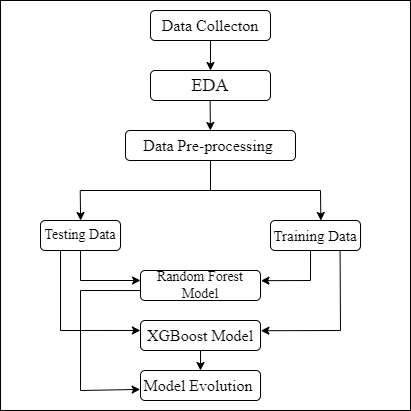
\includegraphics[width=0.7\linewidth]{fig1.jpg}}
    \caption{Proposed Method for training and evaluating models.}
    \label{fig1}
\end{figure}

This research employs quantitative techniques. This approach is more methodical and calls for the use of quantifiable factors, statistics, or numbers. The goal of quantitative research is to create theoretical, mathematical, and structured models that are related to the issues that need to be looked at in detail. Thus, data, theory, and hypothesis are all mentioned in the quantification approach. This approach is suitable for the study since it makes use of datasets with information on cardiovascular risk. There are multiple phases to this study (Fig.1).


The gathering of datasets is the initial stage. After that, the acquired data sets will go through the EDA (Exploration Data Analysis) stage, which tries to comprehend the data sets' contents. Proceed to the data preprocessing stage after completing EDA. The data will go through multiple processing stages throughout the data preprocessing stage before being divided into training and testing data. Following data sharing, the data enters the phase of model training and evaluation.

\subsection{Demographic and Health Data Overview}
In this dataset, demographic data of individuals is encoded as the variable "sex", and reflects if the subject is a man or a woman. Accordingly, the categorical value "sex" is encoded as "M", male, or "F", female. Understanding demographic attributes like sex is crucial for analyzing cardiovascular risk and making tailored interventions more accurate. The dataset incorporates an assortment of demographic, behavioral, and medical history variables, along with past and contemporary medical measurements, that are used to assess cardiovascular risk. One demographic variable is age, which represents the patient's age, and education, which represents the level of education, which is categorized from 1 to 4. Behavioral variables reference smoking habits, with \texttt{is\_smoking} denoting if the patient currently smokes (coded as "YES" or "NO"), and "Cigs Per Day," which represents the average number of cigarettes smoked per day, is quantified as a continuous variable. The medical history variables include blood pressure medicine, stroke history, hypertensive, and diabetes status (named "BP Meds", "Prevalent Stroke", "Prevalent Hyp", and "Diabetes"), all of which is a nominal variables. Current medical measurements include total cholesterol, systolic blood pressure, diastolic blood pressure, Body Mass Index (BMI), heart rate, and glucose level. The target variable of interest is the 10-year risk of Coronary Heart Disease (CHD), coded as binary where "1" represents a risk ("Yes") and "0" represents no risk ("No"). An understanding of these variables can provide invaluable information on cardiovascular risk assessment and can facilitate both the need to construct predictive models and early intervention and treatment strategies in identifying individuals at risk.


\subsection{EDA (Exploratory Data Analysis)}
Exploratory Data Analysis is the process that seeks to understand the dataset by starting with the relationships between columns as well as the length of the data and the data distribution. It is about trying to understand data sets well to analyze the data sets accurately and clean up our datasets. At this point in Exploratory Data Analysis, you can identify the contents of the data sets together with the outliers, double data, missing values, encoding, and noisy data. After you have processed, and understood the data sets, these data sets and the results should be cleaner. Exploratory Data Analysis can be implemented with various approaches as follows:
Data Collection: At this moment, the data is imported and processed. 
Viewing The Structure of The Data: With this approach, we will aim to understand the data that are to be analyzed seriously.
Selecting Data: At this moment, your goal is to prepare the data for the modeling process, so that you will only have the necessary information in the data.
Modifying Variables: This will ensure that the data and modeling will work.
Identifying Outliers and Missing Data: You are looking for missing data, irregular data, or blank data.

\begin{figure}[H]
    \centerline{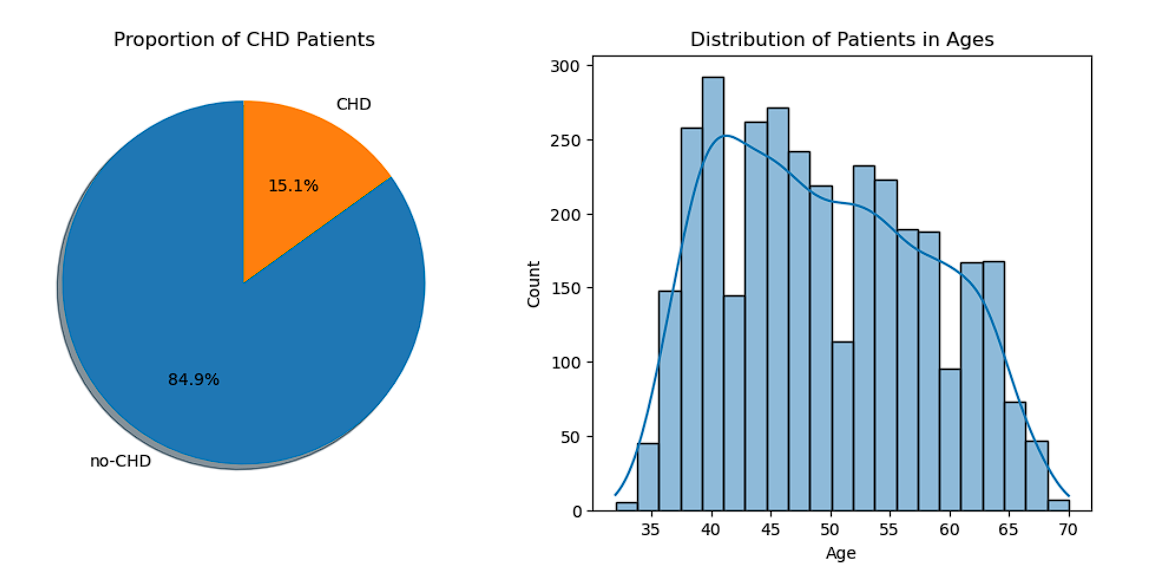
\includegraphics[width=0.7\linewidth]{fig2.png}}
    \caption{Exploratory Data Analysis: Understanding and Preparing the Dataset.}
    \label{fig2}
\end{figure}


About 15\% of individuals in this dataset have a risk of developing CHD in a 10-year interval. The visualization (Fig.2) also has the highest proportion of middle-aged individuals, with the majority in the age group of 40-45 years.

\subsection{Medical History}
\subsubsection{Blood Pressure Medication}

\begin{figure}[H]
    \centerline{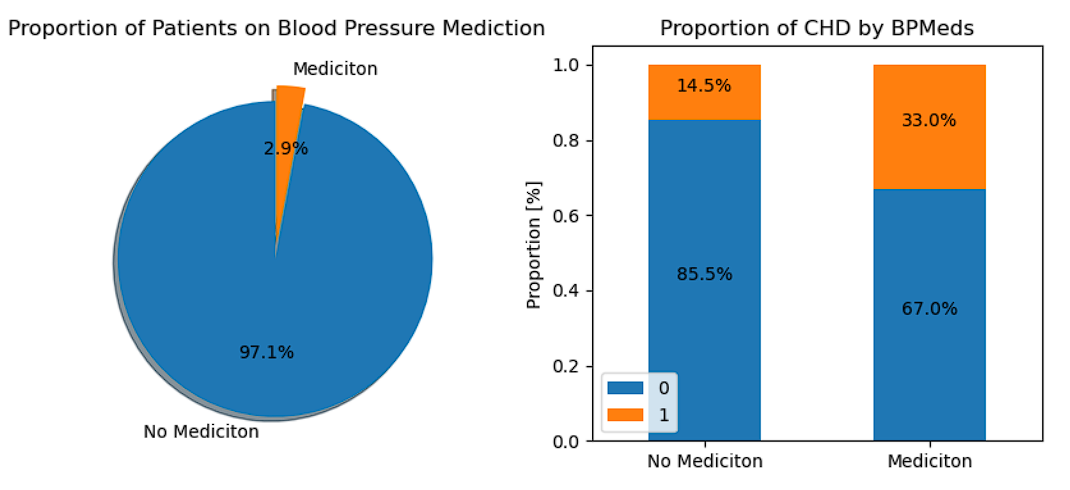
\includegraphics[width=0.7\linewidth]{fig3.png}}
    \caption{Blood Pressure Medication.}
    \label{fig3}
\end{figure}

It can be seen in the given bar charts (Fig.3) that the patients who are prescribed blood pressure medication, have a history of stroke or hypertension, and who also have diabetes are about twice as much as patients who do not have these conditions. However, when examining the information provided in the pie charts, it is important to mention that there are significantly fewer samples of patients who are prescribed blood pressure medication, have diabetes, or have a stroke than there are samples of hypertensive patients. This imbalance in sample sizes could affect the interpretation of the data.

\subsubsection{Blood Pressure Medication}

\begin{figure}[H]
    \centerline{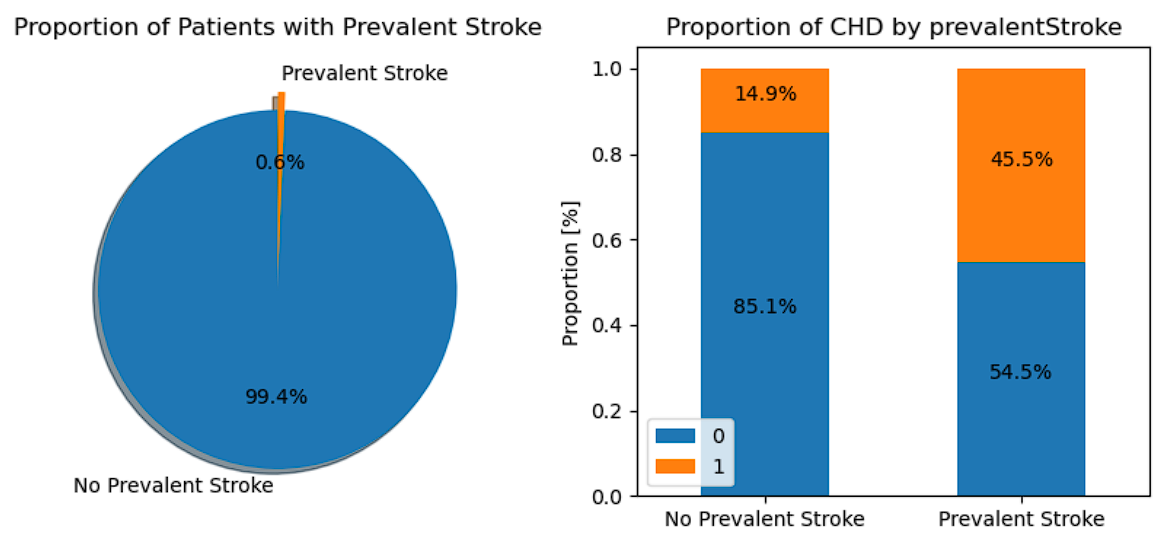
\includegraphics[width=0.7\linewidth]{fig4.png}}
    \caption{Prevalent Stroke.}
    \label{fig4}
\end{figure}

It has been observed that individuals who have a prevalent stroke (Fig.4) are at an elevated risk of developing CHD, up to three times as likely as those without a prevalent stroke. Nonetheless, based on the class of individuals with a prevalent stroke, it is clear that there is an extremely under-represented categorical distribution, accounting for fewer than 1\% of all samples. Since this class has so few represented samples, this attribute will not be incorporated in this present study for training the model due to the potential for biased and inaccurate predictions.

\subsubsection{Prevalent Hypertension}

\begin{figure}[H]
    \centerline{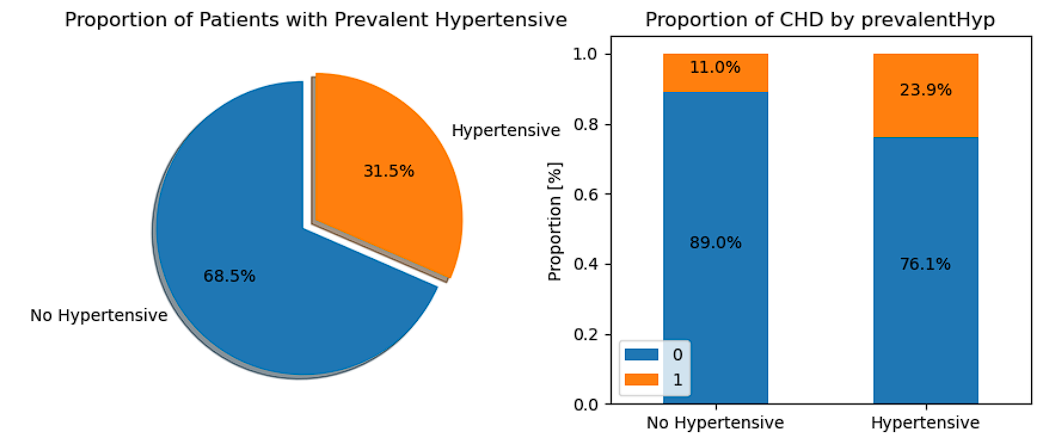
\includegraphics[width=0.7\linewidth]{fig5.png}}
    \caption{Prevalent Hypertension.}
    \label{fig5}
\end{figure}

In the pie chart (Fig.5), it is clear that about thirty-three percent of the patients in this dataset have prevalent hypertension. Additionally, analysis of the histogram indicates that patients who have prevalent hypertension are about two times as likely as patients without hypertension to develop coronary heart disease (CHD).

\subsubsection{Exploratory Analysis of Blood Pressure, Cholesterol Level, and BMI}

Based on this scatter plot, a large portion of people in this dataset have a risk for hypertension because of the high values for systolic and diastolic blood pressure. By estimating the scatter plot, hypertension appears to be prevalent among the participants. The bar chart helps illustrate the relationship between hypertension risk categories and the rate of CHD. It confirms that as the risk of hypertension increases, the CHD rate increases. This is a positive relationship between hypertension and CHD (Fig.6- a). The histogram is beneficial to divide the readings into three categories: healthy levels, risk levels with the highest number of samples, and dangerous levels from the high cholesterol total. The categories permit a better understanding of the distribution of cholesterol readings among the samples and the number of people in different risk levels. The pie chart shows that approximately 20\% of the total samples tested have a healthy level of Cholesterol level. It implies that the majority of the people tested in this analysis are at risk for Hyperlipidemia. CHD rate by Cholesterol level shows a higher cholesterol level increases the CHD rate. The bar chart draws a relationship between the trend of increasing CHD rates and the progress in cholesterol levels. It also shows that the relationship in the bar chart is the same as blood pressure levels, so there is a connection between these two factors (Fig.6-b). The majority of individuals in this dataset were found to be healthy, as indicated by the distribution histogram. However, a significant proportion of the individuals are classified as overweight. The pie chart also indicates a proportion greater than 40\% each for the categories of Healthy and Overweight, with a lower percentage of individuals classified as underweight. The analysis using the histogram suggests a positive relationship between the level of weight and the rate of Coronary Heart Disease (CHD). As weight increases, the rate of CHD also increases. The underweight category demonstrates a CHD rate that appears to be similar to the obese category. This result suggests a potential risk of CHD among individuals classified as underweight. 

\begin{figure}[H]
    \centering
    \begin{subfigure}[b]{0.3\textwidth}
        \centering
        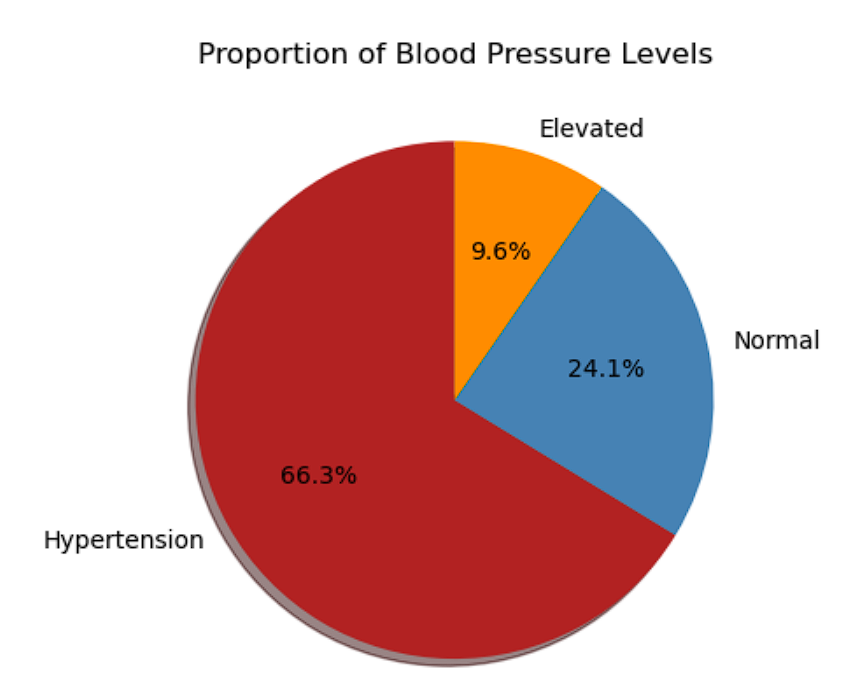
\includegraphics[width=\textwidth]{fig6a.png}
        \caption{}
    \end{subfigure}
    \hfill
    \begin{subfigure}[b]{0.5\textwidth}
        \centering
        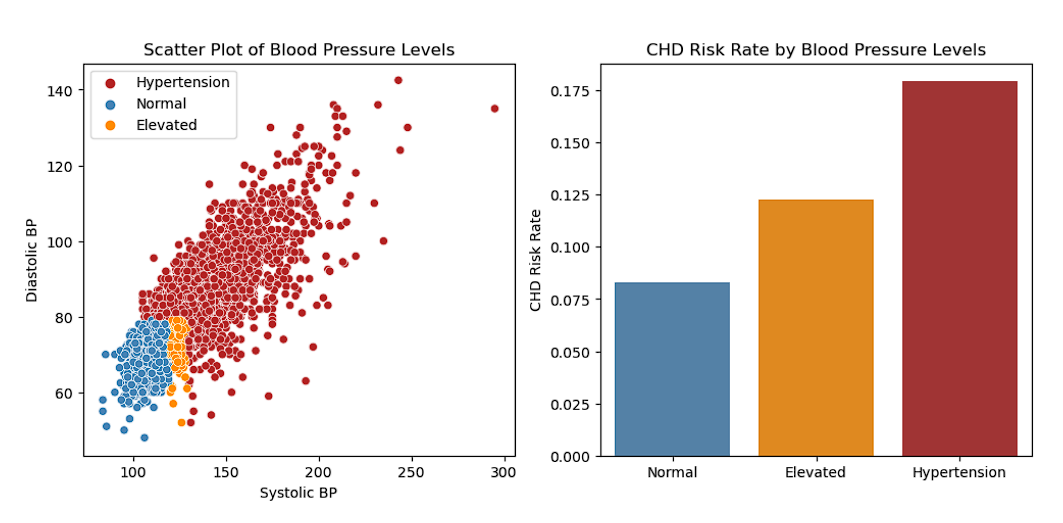
\includegraphics[width=\textwidth]{fig6b.png}
        \caption{}
    \end{subfigure}
    \hfill
    \begin{subfigure}[b]{0.5\textwidth}
        \centering
        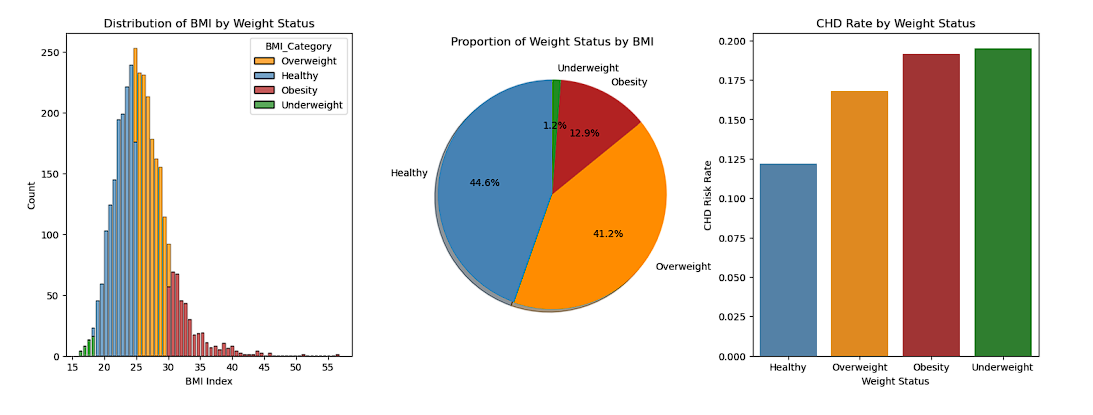
\includegraphics[width=\textwidth]{fig6c.png}
        \caption{}
    \end{subfigure}
    \caption{Exploratory Analysis of Blood Pressure, Cholesterol Level, and BMI}
    \label{fig:exploratory_analysis}
\end{figure}

The sample size for underweight individuals is considerably lower (1.2\%) than the total sample number. As a result, there is less certainty around this finding. Having only 144 underweight individuals may create bias and noise and so the relationship demonstrated in this category may not be as substantiated as other relationships (Fig.6-c).

\subsection{Data Preprocessing}
\subsubsection{Separate Data}
In removing the less pertinent attributes from the data frame, 'is\_smoking', 'cigsPerDay', 'TenYearCHD' will be dropped. In addition, 'prevalentStroke' will also be dropped due to the significant class imbalance in the data.  

\subsubsection{One-Hot Encoder}
One-hot encoding is used to encode categorical variables such as education, sex, BPMeds, prevalentHyp, and diabetes. The database is one-hot encoded using pandas' get\_dummies() method. get\_dummies creates binary columns for each category within each specified categorical variable. Before implementing one-hot encoding, the database is (3390, 12). The dataset expands to (3390, 18) after one-hot encoding, with binary columns representing each category being added. The resulting data frame displays the original variables and their corresponding one-hot encoded binary columns.

\subsubsection{Data Normalization}
The dataset undergoes normalization using the StandardScaler from sklearn.preprocessing module. This process standardizes the features by removing the mean and scaling to unit variance. The transformed dataset, denoted as X\_transform, is represented as an array. Each row corresponds to an individual sample, while each column represents a feature after normalization. Normalization ensures that all features have a mean of 0 and a standard deviation of 1, facilitating better convergence and performance of machine learning models.

\subsubsection{Sampling}
As the Medical History dataset contains several severely imbalanced classes, we used the ADASYN resampling technique to handle the class imbalance issue. By creating new samples, ADASYN helps us learn from the scarce data and overcome the challenges brought by the imbalanced class distribution.

\subsubsection{Models and Evaluation}
The Random Forest and XGBoost models will be used in my data science project to handle the many categories within my attributes. These are models that are well known for their capabilities in classification and regression tasks. Random Forest uses multiple trees to create its predictions producing more consistent outcomes, while XGBoost optimises decision trees to enhance its predictive performance. I chose to use these models to tackle attributes with many categories within my dataset to ensure I get the most reliable and accurate prediction.
In the preprocessing of the data (depicted in Fig.7), non-informative or imbalanced classes attributes, such as "is\_smoking", "cigsPerDay", "TenYearCHD", and "prevalentStroke", are removed. Categorical variables are one-hot encoded to expand the dataset. The raw data is normalized to standardize features and ensure the data is mean-centered with unit variance. Due to the severe class imbalance, the data is resampled using ADASYN.

\begin{figure}[H]
    \centerline{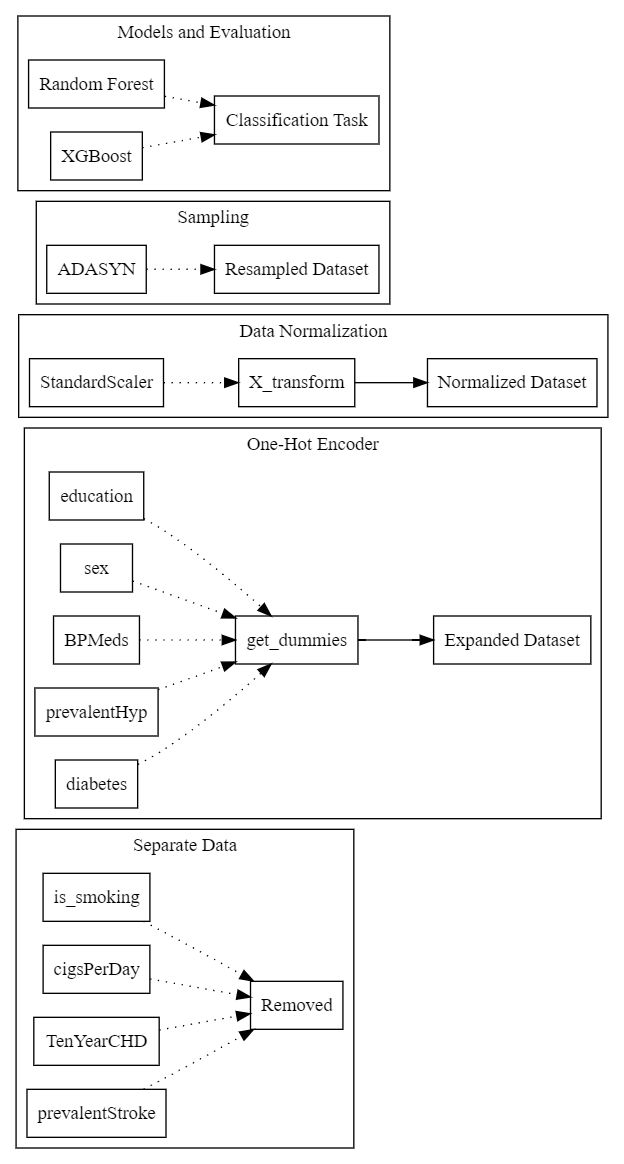
\includegraphics[width=0.7\linewidth]{fig7.png}}
    \caption{Data Preprocessing Workflow.}
    \label{fig7}
\end{figure}

  The Random Forest and XGBoost models are selected for classification due to the task having categorical attributes. These steps are very important in increasing the increased the quality of data and the performance of the model.

  \section{Results And Discussion}

  \subsection{Classification Report}
  
  After EDA, preprocessing, and modeling, we tested the model. The table below shows the performance metrics of the model.
  
  \begin{table}[H]
      \centering
      \caption{Model Performance Metrics}
      \begin{tabularx}{\linewidth}{
          | >{\hsize=1.5\hsize}X
          | >{\hsize=0.8\hsize}X
          | >{\hsize=0.8\hsize}X
          | >{\hsize=0.8\hsize}X
          | >{\hsize=0.8\hsize}X
          | >{\hsize=0.8\hsize}X
          | >{\hsize=0.5\hsize}X |
      }
      \hline
      Model & Accuracy & Jaccard Index & Precision & Recall & F1 Score \\
      \hline
      Random Forest & 0.85 & 0.07 & 0.47 & 0.08 & 0.13 \\ \hline
      XGBoost & 0.82 & 0.09 & 0.29 & 0.12 & 0.17 \\
      \hline
      Random Forest & 0.79 & 0.68 & 0.77 & 0.87 & 0.81 \\ \hline
      XGBoost & 0.79 & 0.66 & 0.80 & 0.79 & 0.79 \\
      \hline
      \end{tabularx}
  \end{table}
  
  The results show that sampling techniques improve model performance on imbalanced datasets. However, the Jaccard index needs improvement.
  
  \subsection{Confusion Matrix}
  
  \begin{figure}[H]
      \begin{minipage}{0.5\linewidth}
          \centering
          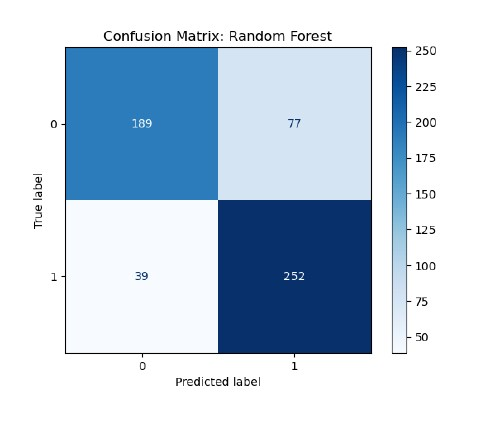
\includegraphics[width=\linewidth]{fig8.jpg}
          \subcaption{Random Forest.}
          \label{fig8}
      \end{minipage}%
      \begin{minipage}{0.5\linewidth}
          \centering
          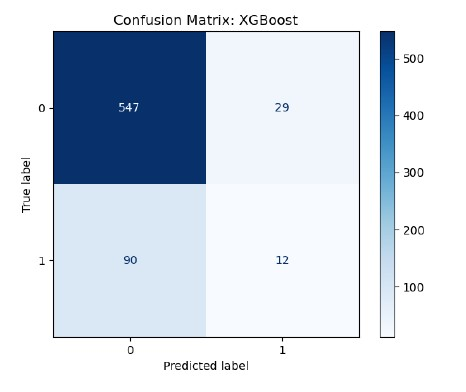
\includegraphics[width=\linewidth]{fig9.jpg}
          \subcaption{XGBoost.}
          \label{fig9}
      \end{minipage}
      \caption{Confusion Matrices for Random Forest and XGBoost.}
  \end{figure}
  
  The confusion matrix shows that sampling techniques improve model performance. However, further optimization is needed to balance precision and recall.
  
  \subsection{Precision-Recall Curve}
  
  \begin{figure}[ht]
  \centering
  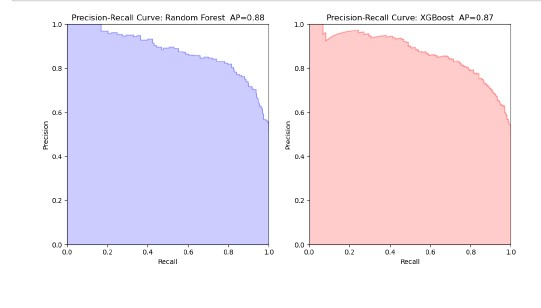
\includegraphics[width=0.8\linewidth]{fig10.jpg}
  \caption{Precision-Recall Curve.}
  \label{fig10}
  \end{figure}
  
  The Precision-Recall Curve shows that precision changes consistently as recall varies.
  
  \section{Optimization}
  
  We tuned the ratio of the oversample using ADASYN sampling and plotted the precision-recall curve for each ratio threshold.
  
  \begin{figure}[ht]
      \centering
      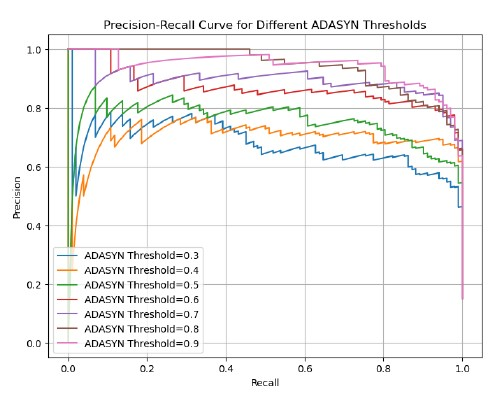
\includegraphics[width=\linewidth]{fig11.jpg}
      \caption{Precision-Recall Curve for Different ADASYN Threshold.}
      \label{fig11}
  \end{figure}
  
  The optimal threshold for both models is 0.9. After optimization, both models showed improved accuracy and Jaccard index. The Random Forest model has a higher recall, while the XGBoost model has a higher precision.

\section{Conclusion}
In conclusion, the evaluation of the models on both sampled and unsampled data revealed that the sampled data consistently outperformed the unsampled data in terms of precision, recall, and overall performance. The sampled data, obtained through techniques such as ADASYN and Random Under Sampling, effectively balanced the class distribution and mitigated the impact of class imbalance.
Comparing the Random Forest and XGBoost models, both models demonstrated similar outcomes in the F1 score. However, the XGBoost model exhibited higher precision, indicating a lower rate of False Positives (Type I error) and a reduced risk of misdiagnosis Therefore, based on the objective of reducing misdiagnosis and ensuring a high precision rate, the XGBoost model would be the preferred option for predicting CHD risk in patients.

\begin{thebibliography}{00}
\bibitem{b1} Arsalan, Khan., Moiz, Qureshi., Muhammad, Daniyal., Kassim, Tawiah. (2023). A Novel Study on Machine Learning Algorithm-Based Cardiovascular Disease Prediction. Health \& Social Care in The Community,  doi: 10.1155/2023/1406060
\bibitem{b2} Kamran, Mehrabani-Zeinabad., Awat, Feizi., Masoumeh, Sadeghi., Hamidreza, Roohafza., Mohammad, Talaei., Nizal, Sarrafzadegan. (2023). Cardiovascular disease incidence prediction by machine learning and statistical techniques: a 16-year cohort study from eastern Mediterranean region. BMC Medical Informatics and Decision Making,  doi: 10.1186/s12911-023-02169-5
\bibitem{b3} Xi, Wei., Cong, Jun, Rao., Xi, Sheng, Xiao., Lin, Chen., Mark, Goh. (2023). Risk assessment of cardiovascular disease based on SOLSSA-CatBoost model. Expert systems with applications,  doi: 10.1016/j.eswa.2023.119648
\bibitem{b4} Weber, Liu., Liliana, Laranjo., Harry, Klimis., Jason, Chiang., Jason, Yue., Simone, Marschner., Juan, C., Quiroz., Louisa, Jorm., Clara, K, Chow. (2023). Machine-learning versus traditional approaches for atherosclerotic cardiovascular risk prognostication in primary prevention cohorts: a systematic review and meta-analysis. European Heart Journal - Quality of Care and Clinical Outcomes,  doi: 10.1093/ehjqcco/qcad017
\bibitem{b5} Elias, Dritsas., Maria, Trigka. (2023). Efficient Data-Driven Machine Learning Models for Cardiovascular Diseases Risk Prediction. Sensors,  doi: 10.3390/s23031161
\bibitem{b6} Rahman, M. A., Noor, R. M., Mallik, S., Santa, N. K., Deb, S., \& Pathak, A. Classification Of Health Risk Levels For Pregnant Women Using Support Vector Machine (SVM) Algorithm.

\end{thebibliography}

\end{document}
